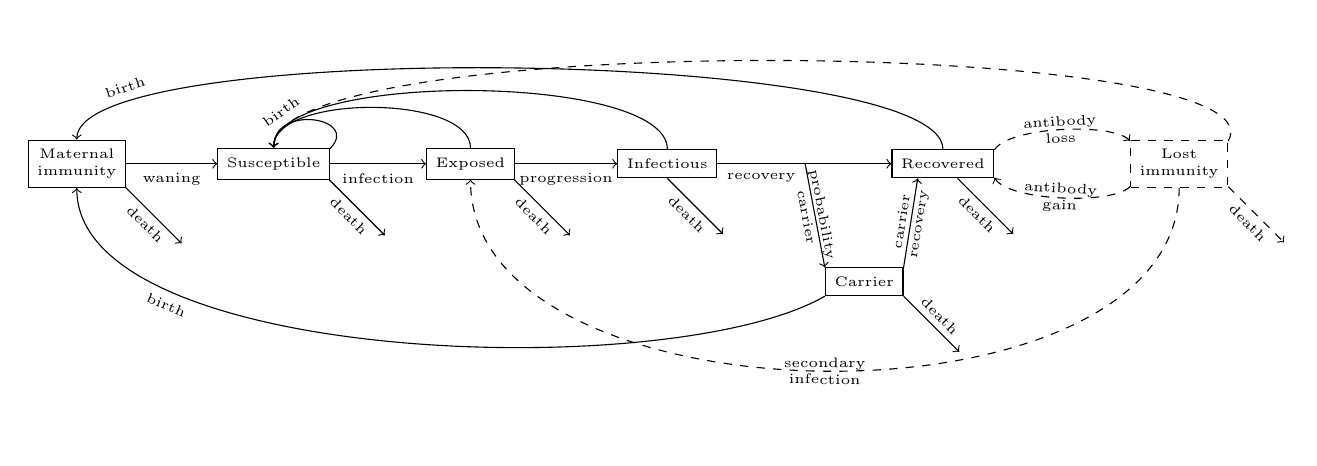
\begin{tikzpicture}[compartment/.style = {rectangle, draw}, font=\fontsize{5pt}{6}\selectfont]
  % Compartments.
  \node at (0, 1.5) [compartment, align=center, name=MaternalImmunity] {Maternal\\immunity};
  \node at (2.5, 1.5) [compartment, name=Susceptible] {Susceptible};
  \node at (5, 1.5) [compartment, name=Exposed] {Exposed};
  \node at (7.5, 1.5) [compartment, name=Infectious] {Infectious};
  \node at (10, 0) [compartment, name=Carrier] {Carrier};
  \node at (11, 1.5) [compartment, name=Recovered] {Recovered};
  \node at (14, 1.5) [compartment, align=center, dashed, name=LostImmunity] {Lost\\immunity};

  % Location for branch from Infectious to Carrier and Recovered.
  \coordinate (recovery) at (9.25, 1.5);

  % Infection-related processes.
  \draw [->] (MaternalImmunity)
             to node [below] {waning}
             (Susceptible);
  \draw [->] (Susceptible)
             to node [below] {infection}
             (Exposed);
  \draw [->] (Exposed)
             to node [below] {progression}
             (Infectious);
  \draw [  ] (Infectious)
             to node [below] {recovery}
             (recovery);
  \draw [->] (recovery)
             to node [sloped, align=center] {probability\\carrier}
             (Carrier.160);
  \draw [->] (recovery)
             to node [] {}
             (Recovered.180);
  \draw [->] (Carrier.20)
             to node [sloped, align=center] {carrier\\recovery}
             (Recovered.210);
  \draw [->, dashed] (Recovered.15)
             to [out=60, in=135, looseness=0.5] node [sloped, align=center] {antibody\\loss}
             (LostImmunity.155);
  \draw [->, dashed] (LostImmunity.205)
             to [out=225, in=300, looseness=0.5] node [sloped, align=center] {antibody\\gain}
             (Recovered.345);
  \draw [->, dashed] (LostImmunity.270)
             to [out=270, in=270, looseness=0.9] node [sloped, align=center] {secondary\\infection}
             (Exposed.270);

  % Births
  \draw [->] (Susceptible.15)
             to [out=45, in=90, looseness=2] node [] {}
             (Susceptible.90);
  \draw [->] (Exposed.90)
             to [out=90, in=90, looseness=0.7] node [] {}
             (Susceptible.90);
  \draw [->] (Infectious.90)
             to [out=90, in=90, looseness=0.5] node [sloped, above, pos=0.88] {birth}
             (Susceptible.90);
  \draw [->] (Carrier.200)
             to [out=210, in=270, looseness=0.6] node [sloped, below, pos=0.75] {birth}
             (MaternalImmunity.270);
  \draw [->] (Recovered.90)
             to [out=90, in=90, looseness=0.3] node [sloped, above, pos=0.85] {birth}
             (MaternalImmunity.90);
  \draw [->, dashed] (LostImmunity.25)
             to [out=60, in=90, looseness=0.32] node [] {}
             (Susceptible.90);

  % Deaths
  \draw [->] (MaternalImmunity.334)
             to node [sloped, below, yshift=1pt] {death}
             +(315: 1);
  \draw [->] (Susceptible.344)
             to node [sloped, below, yshift=1pt] {death}
             +(315: 1);
  \draw [->] (Exposed.340)
             to node [sloped, below, yshift=1pt] {death}
             +(315: 1);
  \draw [->] (Infectious.270)
             to node [sloped, below, yshift=1pt] {death}
             +(315: 1);
  \draw [->] (Carrier.340)
             to node [sloped, above, yshift=-1pt] {death}
             +(315: 1);
  \draw [->] (Recovered.315)
             to node [sloped, below, yshift=1pt] {death}
             +(315: 1);
  \draw [->, dashed] (LostImmunity.335)
             to node [sloped, below, yshift=1pt] {death}
             +(315: 1);
\end{tikzpicture}

%%% Local Variables:
%%% mode: latex
%%% TeX-master: "diagram_horizontal_standalone"
%%% End:
